\documentclass[border=1.5pt]{standalone}
\usepackage{amsmath,amssymb}
\usepackage{tikz}
\usetikzlibrary{arrows.meta,calc,positioning,shapes,shapes.misc,shapes.geometric,backgrounds,fit,decorations.pathreplacing,quantikz2}
% Shared colors and styles for the XYZ^2 figures.
% Pauli types: bright tones for fills and bands, deep (800) shades of the same hues for labels.
% The label shades keep the hue of each Pauli, are well separated from each other (CIEDE2000 > 20)
% and have a contrast ratio of at least 2.9 on the coral cells and 4.5 on the sunflower cells.
\definecolor{PauliX}{HTML}{F97316}
\definecolor{PauliY}{HTML}{EC4899}
\definecolor{PauliZ}{HTML}{9333EA}
\definecolor{PauliXText}{HTML}{AC340B}
\definecolor{PauliYText}{HTML}{9D174D}
\definecolor{PauliZText}{HTML}{5B21B6}
% Generator classes: S0 (class B, even links, coral) and gauge (class A, odd links, sunflower)
\definecolor{Szero}{HTML}{F0435E}
\definecolor{SzeroText}{HTML}{BE123C}
\definecolor{Gauge}{HTML}{F59E0B}
\definecolor{GaugeText}{HTML}{B45309}
\colorlet{GaugeGray}{Gauge}
\definecolor{ClassB}{HTML}{FF8A99}
\definecolor{ClassA}{HTML}{FFD23F}
% Logical operators (X-bar violet, Z-bar crimson), errors, ink
\definecolor{LogicalZ}{HTML}{E11D48}
\definecolor{LogicalGold}{HTML}{7C3AED}
\definecolor{ErrRed}{HTML}{1C1917}
\definecolor{InkDark}{HTML}{292524}
\definecolor{InkSoft}{HTML}{57534E}
% Labels drawn on top of colored cells
\colorlet{CellText}{InkDark}
% Noise channels
\definecolor{ErrFlip}{HTML}{EF4444}
\definecolor{Idle}{HTML}{EC4899}
\definecolor{TwoQ}{HTML}{7C3AED}
% Protocol steps
\definecolor{StepPrep}{HTML}{F97316}
\definecolor{StepMeas}{HTML}{D946EF}
\definecolor{StepDec}{HTML}{7C3AED}
\definecolor{StepRec}{HTML}{DB2777}
\tikzset{
  qb/.style={circle, draw=InkDark, line width=0.6pt, fill=white,
             minimum size=4.2mm, inner sep=0pt, font=\scriptsize},
  qbsmall/.style={circle, draw=InkDark, line width=0.5pt, fill=white,
             minimum size=2.6mm, inner sep=0pt},
  hexedge/.style={line width=0.65pt, draw=InkSoft},
  linkedge/.style={line width=1.6pt, draw=InkDark},
  bndedge/.style={line width=0.65pt, draw=InkSoft, densely dashed},
  plabel/.style={font=\scriptsize\bfseries, inner sep=1pt},
  panel/.style={font=\small\bfseries, anchor=north west},
}

\providecommand{\ket}[1]{\left|#1\right\rangle}

\begin{document}
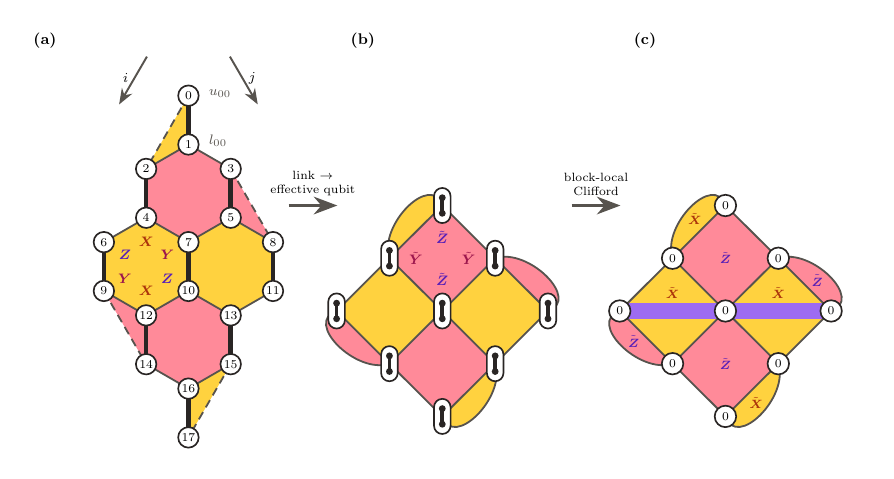
\begin{tikzpicture}[scale=0.62, every node/.style={transform shape}]
\fill[ClassB] (0.000,-0.500) -- (0.866,-1.000) -- (0.866,-2.000) -- (0.000,-2.500) -- (-0.866,-2.000) -- (-0.866,-1.000) -- cycle;
\fill[ClassA] (0.866,-2.000) -- (1.732,-2.500) -- (1.732,-3.500) -- (0.866,-4.000) -- (0.000,-3.500) -- (0.000,-2.500) -- cycle;
\fill[ClassA] (-0.866,-2.000) -- (0.000,-2.500) -- (0.000,-3.500) -- (-0.866,-4.000) -- (-1.732,-3.500) -- (-1.732,-2.500) -- cycle;
\fill[ClassB] (0.000,-3.500) -- (0.866,-4.000) -- (0.866,-5.000) -- (0.000,-5.500) -- (-0.866,-5.000) -- (-0.866,-4.000) -- cycle;
\fill[ClassA] (-0.866,-1.000) -- (0.000,-0.500) -- (0.000,0.500) -- cycle;
\fill[ClassB] (-0.866,-5.000) -- (-0.866,-4.000) -- (-1.732,-3.500) -- cycle;
\fill[ClassB] (0.866,-2.000) -- (1.732,-2.500) -- (0.866,-1.000) -- cycle;
\fill[ClassA] (0.000,-6.500) -- (0.866,-5.000) -- (0.000,-5.500) -- cycle;
\draw[hexedge] (0.000,-0.500) -- (-0.866,-1.000);
\draw[hexedge] (0.000,-0.500) -- (0.866,-1.000);
\draw[hexedge] (-0.866,-1.000) -- (-0.866,-2.000);
\draw[hexedge] (0.866,-1.000) -- (0.866,-2.000);
\draw[hexedge] (-0.866,-2.000) -- (-1.732,-2.500);
\draw[hexedge] (-0.866,-2.000) -- (0.000,-2.500);
\draw[hexedge] (0.866,-2.000) -- (0.000,-2.500);
\draw[hexedge] (0.866,-2.000) -- (1.732,-2.500);
\draw[hexedge] (-1.732,-2.500) -- (-1.732,-3.500);
\draw[hexedge] (0.000,-2.500) -- (0.000,-3.500);
\draw[hexedge] (1.732,-2.500) -- (1.732,-3.500);
\draw[hexedge] (-1.732,-3.500) -- (-0.866,-4.000);
\draw[hexedge] (0.000,-3.500) -- (-0.866,-4.000);
\draw[hexedge] (0.000,-3.500) -- (0.866,-4.000);
\draw[hexedge] (1.732,-3.500) -- (0.866,-4.000);
\draw[hexedge] (-0.866,-4.000) -- (-0.866,-5.000);
\draw[hexedge] (0.866,-4.000) -- (0.866,-5.000);
\draw[hexedge] (-0.866,-5.000) -- (0.000,-5.500);
\draw[hexedge] (0.866,-5.000) -- (0.000,-5.500);
\draw[bndedge] (0.000,0.500) -- (-0.866,-1.000);
\draw[bndedge] (-1.732,-3.500) -- (-0.866,-5.000);
\draw[bndedge] (0.866,-1.000) -- (1.732,-2.500);
\draw[bndedge] (0.866,-5.000) -- (0.000,-6.500);
\draw[linkedge, draw=InkDark] (0.000,0.500) -- (0.000,-0.500);
\draw[linkedge, draw=InkDark] (0.866,-1.000) -- (0.866,-2.000);
\draw[linkedge, draw=InkDark] (1.732,-2.500) -- (1.732,-3.500);
\draw[linkedge, draw=InkDark] (-0.866,-1.000) -- (-0.866,-2.000);
\draw[linkedge, draw=InkDark] (0.000,-2.500) -- (0.000,-3.500);
\draw[linkedge, draw=InkDark] (0.866,-4.000) -- (0.866,-5.000);
\draw[linkedge, draw=InkDark] (-1.732,-2.500) -- (-1.732,-3.500);
\draw[linkedge, draw=InkDark] (-0.866,-4.000) -- (-0.866,-5.000);
\draw[linkedge, draw=InkDark] (0.000,-5.500) -- (0.000,-6.500);

\node[qb, fill=white] (q0) at (0.000,0.500) {0};
\node[qb, fill=white] (q1) at (0.000,-0.500) {1};
\node[qb, fill=white] (q2) at (-0.866,-1.000) {2};
\node[qb, fill=white] (q3) at (0.866,-1.000) {3};
\node[qb, fill=white] (q4) at (-0.866,-2.000) {4};
\node[qb, fill=white] (q5) at (0.866,-2.000) {5};
\node[qb, fill=white] (q6) at (-1.732,-2.500) {6};
\node[qb, fill=white] (q7) at (0.000,-2.500) {7};
\node[qb, fill=white] (q8) at (1.732,-2.500) {8};
\node[qb, fill=white] (q9) at (-1.732,-3.500) {9};
\node[qb, fill=white] (q10) at (0.000,-3.500) {10};
\node[qb, fill=white] (q11) at (1.732,-3.500) {11};
\node[qb, fill=white] (q12) at (-0.866,-4.000) {12};
\node[qb, fill=white] (q13) at (0.866,-4.000) {13};
\node[qb, fill=white] (q14) at (-0.866,-5.000) {14};
\node[qb, fill=white] (q15) at (0.866,-5.000) {15};
\node[qb, fill=white] (q16) at (0.000,-5.500) {16};
\node[qb, fill=white] (q17) at (0.000,-6.500) {17};
\node[plabel, text=PauliXText, font=\footnotesize] at (-0.866,-2.500) {$\boldsymbol{X}$};
\node[plabel, text=PauliZText, font=\footnotesize] at (-1.299,-2.750) {$\boldsymbol{Z}$};
\node[plabel, text=PauliYText, font=\footnotesize] at (-0.433,-2.750) {$\boldsymbol{Y}$};
\node[plabel, text=PauliYText, font=\footnotesize] at (-1.299,-3.250) {$\boldsymbol{Y}$};
\node[plabel, text=PauliZText, font=\footnotesize] at (-0.433,-3.250) {$\boldsymbol{Z}$};
\node[plabel, text=PauliXText, font=\footnotesize] at (-0.866,-3.500) {$\boldsymbol{X}$};

\fill[ClassB] (7.365,-3.910) .. controls (8.048,-3.683) and (6.966,-2.603) .. (6.283,-2.830) -- cycle;
\draw[hexedge] (7.365,-3.910) .. controls (8.048,-3.683) and (6.966,-2.603) .. (6.283,-2.830);
\fill[ClassA] (5.200,-1.750) .. controls (4.972,-1.067) and (3.889,-2.147) .. (4.117,-2.830) -- cycle;
\draw[hexedge] (5.200,-1.750) .. controls (4.972,-1.067) and (3.889,-2.147) .. (4.117,-2.830);
\fill[ClassB] (5.200,-1.750) -- (6.283,-2.830) -- (5.200,-3.910) -- (4.117,-2.830) -- cycle;
\fill[ClassA] (6.283,-2.830) -- (7.365,-3.910) -- (6.283,-4.990) -- (5.200,-3.910) -- cycle;
\fill[ClassA] (4.117,-2.830) -- (5.200,-3.910) -- (4.117,-4.990) -- (3.035,-3.910) -- cycle;
\fill[ClassB] (5.200,-3.910) -- (6.283,-4.990) -- (5.200,-6.070) -- (4.117,-4.990) -- cycle;
\fill[ClassA] (6.283,-4.990) .. controls (6.511,-5.673) and (5.428,-6.753) .. (5.200,-6.070) -- cycle;
\draw[hexedge] (6.283,-4.990) .. controls (6.511,-5.673) and (5.428,-6.753) .. (5.200,-6.070);
\fill[ClassB] (3.035,-3.910) .. controls (2.352,-4.137) and (3.434,-5.217) .. (4.117,-4.990) -- cycle;
\draw[hexedge] (3.035,-3.910) .. controls (2.352,-4.137) and (3.434,-5.217) .. (4.117,-4.990);
\draw[hexedge] (5.200,-1.750) -- (6.283,-2.830);
\draw[hexedge] (5.200,-1.750) -- (4.117,-2.830);
\draw[hexedge] (6.283,-2.830) -- (7.365,-3.910);
\draw[hexedge] (6.283,-2.830) -- (5.200,-3.910);
\draw[hexedge] (7.365,-3.910) -- (6.283,-4.990);
\draw[hexedge] (4.117,-2.830) -- (5.200,-3.910);
\draw[hexedge] (4.117,-2.830) -- (3.035,-3.910);
\draw[hexedge] (5.200,-3.910) -- (6.283,-4.990);
\draw[hexedge] (5.200,-3.910) -- (4.117,-4.990);
\draw[hexedge] (6.283,-4.990) -- (5.200,-6.070);
\draw[hexedge] (3.035,-3.910) -- (4.117,-4.990);
\draw[hexedge] (4.117,-4.990) -- (5.200,-6.070);
\node[draw=InkDark, line width=0.6pt, fill=white, rounded rectangle, rotate=90, minimum width=7.2mm, minimum height=3.4mm, inner sep=0pt] at (5.200,-1.750) {};
\draw[line width=1.3pt, draw=InkDark] (5.200,-1.590) -- (5.200,-1.910);
\fill[InkDark] (5.200,-1.590) circle (0.07);
\fill[InkDark] (5.200,-1.910) circle (0.07);
\node[draw=InkDark, line width=0.6pt, fill=white, rounded rectangle, rotate=90, minimum width=7.2mm, minimum height=3.4mm, inner sep=0pt] at (6.283,-2.830) {};
\draw[line width=1.3pt, draw=InkDark] (6.283,-2.670) -- (6.283,-2.990);
\fill[InkDark] (6.283,-2.670) circle (0.07);
\fill[InkDark] (6.283,-2.990) circle (0.07);
\node[draw=InkDark, line width=0.6pt, fill=white, rounded rectangle, rotate=90, minimum width=7.2mm, minimum height=3.4mm, inner sep=0pt] at (7.365,-3.910) {};
\draw[line width=1.3pt, draw=InkDark] (7.365,-3.750) -- (7.365,-4.070);
\fill[InkDark] (7.365,-3.750) circle (0.07);
\fill[InkDark] (7.365,-4.070) circle (0.07);
\node[draw=InkDark, line width=0.6pt, fill=white, rounded rectangle, rotate=90, minimum width=7.2mm, minimum height=3.4mm, inner sep=0pt] at (4.117,-2.830) {};
\draw[line width=1.3pt, draw=InkDark] (4.117,-2.670) -- (4.117,-2.990);
\fill[InkDark] (4.117,-2.670) circle (0.07);
\fill[InkDark] (4.117,-2.990) circle (0.07);
\node[draw=InkDark, line width=0.6pt, fill=white, rounded rectangle, rotate=90, minimum width=7.2mm, minimum height=3.4mm, inner sep=0pt] at (5.200,-3.910) {};
\draw[line width=1.3pt, draw=InkDark] (5.200,-3.750) -- (5.200,-4.070);
\fill[InkDark] (5.200,-3.750) circle (0.07);
\fill[InkDark] (5.200,-4.070) circle (0.07);
\node[draw=InkDark, line width=0.6pt, fill=white, rounded rectangle, rotate=90, minimum width=7.2mm, minimum height=3.4mm, inner sep=0pt] at (6.283,-4.990) {};
\draw[line width=1.3pt, draw=InkDark] (6.283,-4.830) -- (6.283,-5.150);
\fill[InkDark] (6.283,-4.830) circle (0.07);
\fill[InkDark] (6.283,-5.150) circle (0.07);
\node[draw=InkDark, line width=0.6pt, fill=white, rounded rectangle, rotate=90, minimum width=7.2mm, minimum height=3.4mm, inner sep=0pt] at (3.035,-3.910) {};
\draw[line width=1.3pt, draw=InkDark] (3.035,-3.750) -- (3.035,-4.070);
\fill[InkDark] (3.035,-3.750) circle (0.07);
\fill[InkDark] (3.035,-4.070) circle (0.07);
\node[draw=InkDark, line width=0.6pt, fill=white, rounded rectangle, rotate=90, minimum width=7.2mm, minimum height=3.4mm, inner sep=0pt] at (4.117,-4.990) {};
\draw[line width=1.3pt, draw=InkDark] (4.117,-4.830) -- (4.117,-5.150);
\fill[InkDark] (4.117,-4.830) circle (0.07);
\fill[InkDark] (4.117,-5.150) circle (0.07);
\node[draw=InkDark, line width=0.6pt, fill=white, rounded rectangle, rotate=90, minimum width=7.2mm, minimum height=3.4mm, inner sep=0pt] at (5.200,-6.070) {};
\draw[line width=1.3pt, draw=InkDark] (5.200,-5.910) -- (5.200,-6.230);
\fill[InkDark] (5.200,-5.910) circle (0.07);
\fill[InkDark] (5.200,-6.230) circle (0.07);
\node[plabel, text=PauliZText, font=\footnotesize] at (5.200,-2.398) {$\tilde{\boldsymbol{Z}}$};
\node[plabel, text=PauliYText, font=\footnotesize] at (5.741,-2.830) {$\tilde{\boldsymbol{Y}}$};
\node[plabel, text=PauliZText, font=\footnotesize] at (5.200,-3.262) {$\tilde{\boldsymbol{Z}}$};
\node[plabel, text=PauliYText, font=\footnotesize] at (4.659,-2.830) {$\tilde{\boldsymbol{Y}}$};
\fill[ClassB] (13.165,-3.910) .. controls (13.848,-3.683) and (12.766,-2.603) .. (12.083,-2.830) -- cycle;
\draw[hexedge] (13.165,-3.910) .. controls (13.848,-3.683) and (12.766,-2.603) .. (12.083,-2.830);
\fill[ClassA] (11.000,-1.750) .. controls (10.772,-1.067) and (9.689,-2.147) .. (9.917,-2.830) -- cycle;
\draw[hexedge] (11.000,-1.750) .. controls (10.772,-1.067) and (9.689,-2.147) .. (9.917,-2.830);
\fill[ClassB] (11.000,-1.750) -- (12.083,-2.830) -- (11.000,-3.910) -- (9.917,-2.830) -- cycle;
\fill[ClassA] (12.083,-2.830) -- (13.165,-3.910) -- (12.083,-4.990) -- (11.000,-3.910) -- cycle;
\fill[ClassA] (9.917,-2.830) -- (11.000,-3.910) -- (9.917,-4.990) -- (8.835,-3.910) -- cycle;
\fill[ClassB] (11.000,-3.910) -- (12.083,-4.990) -- (11.000,-6.070) -- (9.917,-4.990) -- cycle;
\fill[ClassA] (12.083,-4.990) .. controls (12.311,-5.673) and (11.228,-6.753) .. (11.000,-6.070) -- cycle;
\draw[hexedge] (12.083,-4.990) .. controls (12.311,-5.673) and (11.228,-6.753) .. (11.000,-6.070);
\fill[ClassB] (8.835,-3.910) .. controls (8.152,-4.137) and (9.234,-5.217) .. (9.917,-4.990) -- cycle;
\draw[hexedge] (8.835,-3.910) .. controls (8.152,-4.137) and (9.234,-5.217) .. (9.917,-4.990);
\draw[line width=6pt, draw=LogicalGold!75, line cap=round] (13.165,-3.910) -- (11.000,-3.910) -- (8.835,-3.910);
\draw[hexedge] (11.000,-1.750) -- (12.083,-2.830);
\draw[hexedge] (11.000,-1.750) -- (9.917,-2.830);
\draw[hexedge] (12.083,-2.830) -- (13.165,-3.910);
\draw[hexedge] (12.083,-2.830) -- (11.000,-3.910);
\draw[hexedge] (13.165,-3.910) -- (12.083,-4.990);
\draw[hexedge] (9.917,-2.830) -- (11.000,-3.910);
\draw[hexedge] (9.917,-2.830) -- (8.835,-3.910);
\draw[hexedge] (11.000,-3.910) -- (12.083,-4.990);
\draw[hexedge] (11.000,-3.910) -- (9.917,-4.990);
\draw[hexedge] (12.083,-4.990) -- (11.000,-6.070);
\draw[hexedge] (8.835,-3.910) -- (9.917,-4.990);
\draw[hexedge] (9.917,-4.990) -- (11.000,-6.070);
\node[circle, draw=InkDark, line width=0.6pt, fill=white, minimum size=4.4mm, inner sep=0pt, font=\scriptsize] at (11.000,-1.750) {$0$};
\node[circle, draw=InkDark, line width=0.6pt, fill=white, minimum size=4.4mm, inner sep=0pt, font=\scriptsize] at (12.083,-2.830) {$0$};
\node[circle, draw=InkDark, line width=0.6pt, fill=white, minimum size=4.4mm, inner sep=0pt, font=\scriptsize] at (13.165,-3.910) {$0$};
\node[circle, draw=InkDark, line width=0.6pt, fill=white, minimum size=4.4mm, inner sep=0pt, font=\scriptsize] at (9.917,-2.830) {$0$};
\node[circle, draw=InkDark, line width=0.6pt, fill=white, minimum size=4.4mm, inner sep=0pt, font=\scriptsize] at (11.000,-3.910) {$0$};
\node[circle, draw=InkDark, line width=0.6pt, fill=white, minimum size=4.4mm, inner sep=0pt, font=\scriptsize] at (12.083,-4.990) {$0$};
\node[circle, draw=InkDark, line width=0.6pt, fill=white, minimum size=4.4mm, inner sep=0pt, font=\scriptsize] at (8.835,-3.910) {$0$};
\node[circle, draw=InkDark, line width=0.6pt, fill=white, minimum size=4.4mm, inner sep=0pt, font=\scriptsize] at (9.917,-4.990) {$0$};
\node[circle, draw=InkDark, line width=0.6pt, fill=white, minimum size=4.4mm, inner sep=0pt, font=\scriptsize] at (11.000,-6.070) {$0$};
\node[font=\scriptsize, text=PauliZText] at (12.880,-3.285) {$\tilde{\boldsymbol{Z}}$};
\node[font=\scriptsize, text=PauliXText] at (10.373,-2.034) {$\tilde{\boldsymbol{X}}$};
\node[font=\scriptsize, text=PauliZText] at (11.000,-2.830) {$\tilde{\boldsymbol{Z}}$};
\node[font=\scriptsize, text=PauliXText] at (12.083,-3.550) {$\tilde{\boldsymbol{X}}$};
\node[font=\scriptsize, text=PauliXText] at (9.917,-3.550) {$\tilde{\boldsymbol{X}}$};
\node[font=\scriptsize, text=PauliZText] at (11.000,-4.990) {$\tilde{\boldsymbol{Z}}$};
\node[font=\scriptsize, text=PauliXText] at (11.627,-5.786) {$\tilde{\boldsymbol{X}}$};
\node[font=\scriptsize, text=PauliZText] at (9.120,-4.535) {$\tilde{\boldsymbol{Z}}$};
\draw[-{Stealth[length=3mm]}, line width=0.9pt, draw=InkSoft] (2.05,-1.75) -- (3.05,-1.75) node[midway, above=2pt, font=\scriptsize, align=center] {link $\to$\\ effective qubit};
\draw[-{Stealth[length=3mm]}, line width=0.9pt, draw=InkSoft] (7.85,-1.75) -- (8.85,-1.75) node[midway, above=2pt, font=\scriptsize, align=center] {block-local\\ Clifford};
\node[font=\footnotesize, text=InkSoft, anchor=west] at (0.30,0.55) {$u_{00}$};
\node[font=\footnotesize, text=InkSoft, anchor=west] at (0.30,-0.42) {$l_{00}$};
\draw[-{Stealth[length=2mm]}, line width=0.7pt, draw=InkSoft] (0.85,1.3) -- (1.42,0.32) node[pos=0.45, right, font=\footnotesize] {$j$};
\draw[-{Stealth[length=2mm]}, line width=0.7pt, draw=InkSoft] (-0.85,1.3) -- (-1.42,0.32) node[pos=0.45, left, font=\footnotesize] {$i$};
\node[panel] at (-3.3,1.9) {(a)};
\node[panel] at (3.2,1.9) {(b)};
\node[panel] at (9.0,1.9) {(c)};
\end{tikzpicture}
\end{document}
